\documentclass[12pt,a4paper]{article} \usepackage[utf8]{inputenc} \usepackage[T1]{fontenc} \usepackage[brazil]{babel} \usepackage{geometry} \geometry{a4paper, margin=2.5cm} \usepackage{setspace} \usepackage{graphicx} \usepackage{hyperref} \title{Relatório – Laboratório Introdutório Wireshark} \author{Samuel Abrão - 24101216} \date{\today} \begin{document} \maketitle \section{Resultados} \subsection*{1. Três protocolos identificados antes do filtro HTTP} Na captura original (sem filtros), é possível identificar: \begin{itemize} \item HTTP \item TCP \item Ethernet II \end{itemize} \subsection*{2. Tempo entre o HTTP GET e o HTTP OK} O pacote \texttt{GET} foi identificado como número 5885 e o \texttt{HTTP 200 OK} como número 5928. Pelos registros de tempo, a resposta foi praticamente imediata (menos de 1 segundo). Para precisão absoluta, a diferença deve ser calculada a partir do arquivo de captura original. \subsection*{3. Endereços IP} \begin{itemize} \item IP do servidor \texttt{gaia.cs.umass.edu}: \texttt{128.119.245.12} \item IP da máquina local: \texttt{192.168.43.158} \end{itemize} \begin{figure}[H] \centering 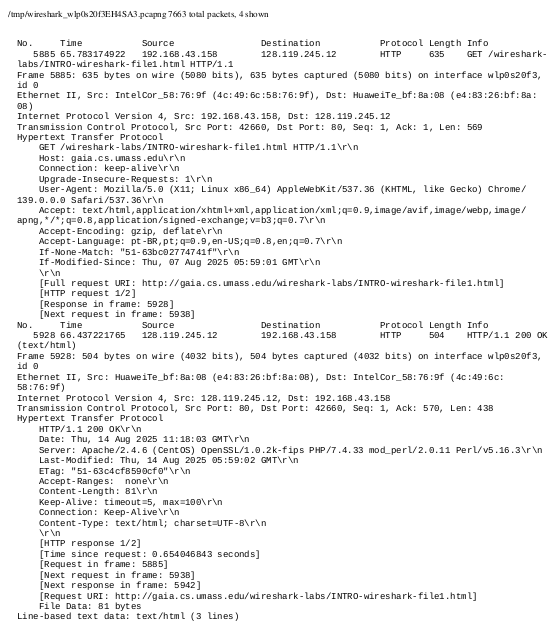
\includegraphics[width=\textwidth]{print.png} \caption{Captura de pacotes HTTP no Wireshark.} \end{figure} \section{Conclusão} O laboratório permitiu a observação prática da estrutura de uma requisição HTTP, desde a camada de enlace (Ethernet II), passando pelas camadas de rede (IP) e transporte (TCP), até a camada de aplicação (HTTP). Também reforçou a importância de compreender a sequência de pacotes e o uso de filtros no Wireshark para análise eficiente. (Print na próxima página) \end{document}